\chapter{Crowdsourcing based Environmental Noise Monitoring System}

\section{Introdution}




\subsection{Noise Pollution}

Sound is essential to our daily lives, but noise is not. Noise can be defined as sounds or noises that are loud, annoying and harmful to the ear.  Loud music, the television, people talking on their phone, the traffic and even pets barking have become a part of the urban culture and rarely disturb us. However, when the sound of the television keeps you from sleeping all night or the traffic starts to give you a headache, it stops becoming just noise and start turning into noise pollution. For many of us, the concept of pollution is limited to nature and resources. However, noise that tends to disrupt the natural rhythm of life makes for one solid pollutant. By definition, noise pollution takes place when there is either excessive amount of noise or an unpleasant sound that causes temporary disruption in the natural balance. Poor urban planning may give rise to noise pollution, since side-by-side industrial and residential buildings can result in noise pollution in the residential areas. 
\\
Noise measurements in urban areas are mainly carried out by designated officers that collect data in a location of interest for successive analysis and storage, using a sound level meter or similar device. This manual collection method using expensive equipment does not scale as the demand for higher granularity of noise measurements in both time and space increases.

\begin{figure}[!htbp]
	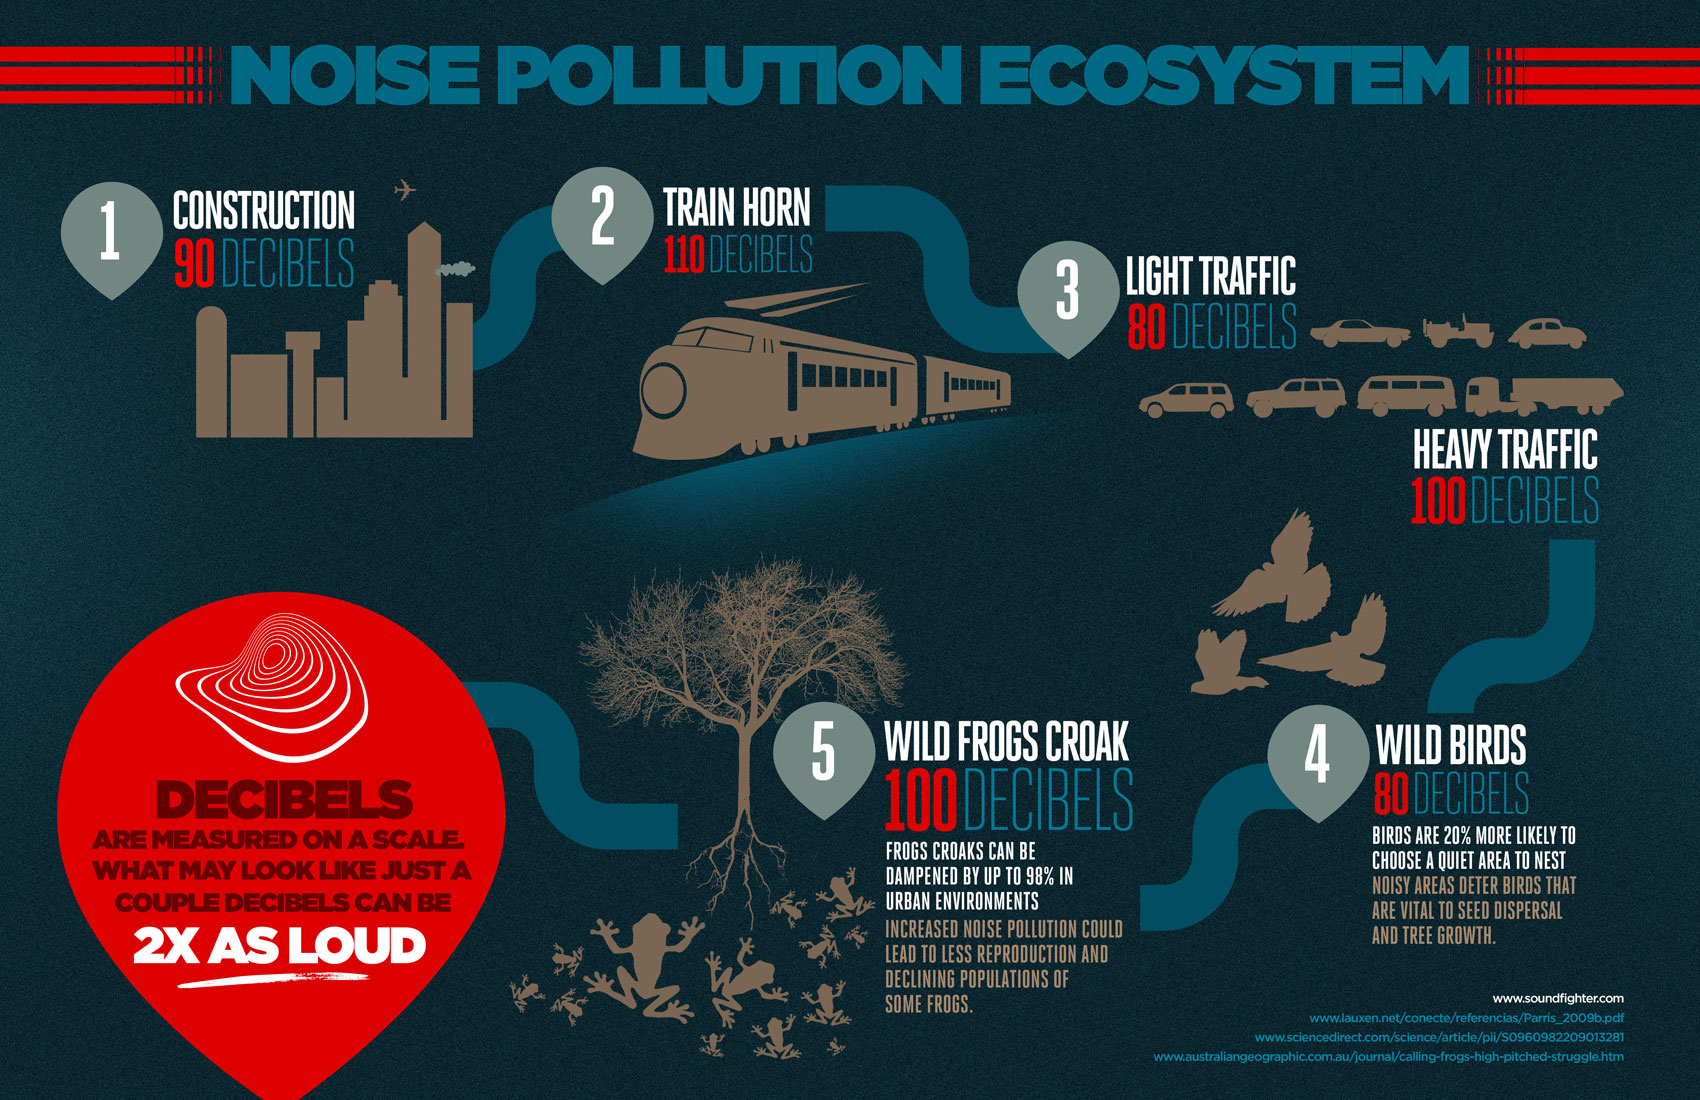
\includegraphics[width=0.8\textwidth]{1.jpg}
	\centering
	\label{fig:Noise Polution}
	\caption{Noise Pollution}
\end{figure}

\subsection{Effects of Noise Pollution}

\begin{itemize}
	\item Excessive noise pollution in working areas such as offices, construction sites, bars and even in our homes can influence psychological health. Studies show that the occurrence of aggressive behavior, disturbance of sleep, constant stress, hypertension can be linked to excessive noise levels.It may lead to problems related to fatigue and your performance may go down in office as well as at home. These in turn can cause more severe and chronic health issues later.
	
	\item Blood pressure levels, cardio-vascular disease and stress related heart problems are on the rise. Studies suggest that high intensity noise causes high blood pressure and increases heart beat rate as it disrupts the normal blood flow. Bringing them to a manageable level depends on our understanding noise pollution and how we tackle it.
	
	\item Wildlife faces far more problems than humans because noise pollution since they are more dependent on sound. Animals develop a better sense of hearing than us since their survival depends on it. The ill effects of excessive noise begin at home. Pets react more aggressively in households where there is constant noise. It has resulted in the declination of diversity of bird species around cities and major roads.
\end{itemize}

\section{Crowd Sourcing}

\begin{figure}[!htbp]
	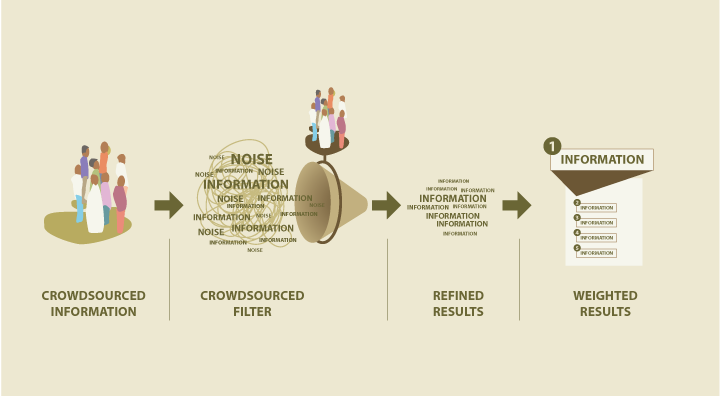
\includegraphics[width=0.8\textwidth]{2.png}
	\centering
	\label{fig:Croud Sourcing}
	\caption{Crowd Sourcing}
\end{figure}

To improve economic and social conditions in urban environments, technicians and urban planners develop infrastructures that connect everyday living to the natural and informational resources to help making cities more sustainable. As population increases, cities become bigger and noisier and excessive noise levels have a direct impact on nature and environment. A new way of acquiring environmental data is by using the concept of “citizens-as-sensors”, also known in literature as crowdsourcing. With the application of this technique, we enable citizens to produce geographic information at a very low cost.

Smartphone penetration has increased dramatically worldwide in recent years.Smartphones are equipped with various imbedded sensors capable of monitoring sound, light, proximity, magnetism, motion, geographic location, and others. It allows ‘crowd sourcing,’ wherein data sensed by the smartphones of anonymous users can provide copious and valuable information. Crowd sourcing is an inexpensive, effective, and efficient means of data collection that overcomes temporal and spatial boundaries.

Although it sounds simple, this turns out to be a task with some precise difficulties. Smartphones can provide accurate measurements of ambient sound as well as a location and time stamp to show exactly where the measurement was taken. The difficulty is in ensuring that the measurements are useful recordings of ambient noise and no other sounds that might distort the readings. Unwanted noises include conversations nearby, which will sound loud but are unlikely to contribute significantly to ambient noise, or the sound of keys or other paraphernalia jangling in a bag or the muffled readings that a phone inside a pocket might produce.

\section{Architecture of the Android Application}


\begin{figure}[!htbp]
	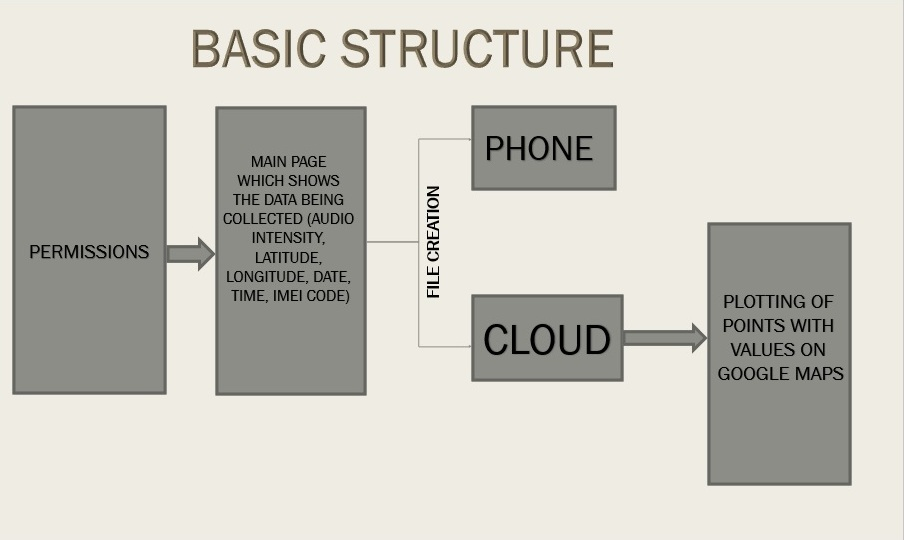
\includegraphics[width=0.8\textwidth]{3.jpg}
	\centering
	\label{fig:Architecture}
	\caption{Architecture}
\end{figure}

The application is installed in the android device. When we open the application, it asks for the permission from various sensors (GPS, Mic, etc). 
The GPS is used to obtain the Latitude and Longitude of thelocation, from where the data is taken. From the location, we get the address of the location.  
The microphone is used to get the noise reading from the surrounding, from the reading we calculate the maximum amplitude from it.
The phone ID is used to get the IMEI number of the android device. 
The memory card permission is used to store the date-time, latitude, longitude, address, amplitude, IMEI number in the SDcard of the Android device.
So, all the data is stored in the SDcard in a.csv file. The app then calls a php file which uploads data into the MySQL database.
From where we can access the data via XML and plot the location marker in the Google Map.The marker shows the date-time, amplitude, address, latitude and longitude on the Google Map.
For all the process to work the necessary condition is that your Android Device should always be connected to the Internet.Otherwise the applicationwillcrash.



\begin{figure}
	\hfill
	\subfigure[Home]{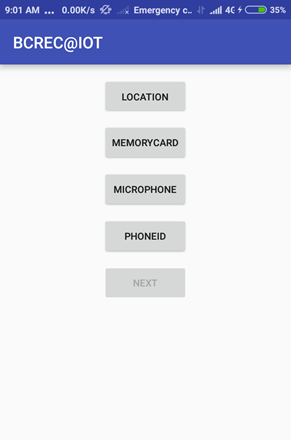
\includegraphics[width=5cm]{4.png}}
	\hfill
	\subfigure[Noise Map]{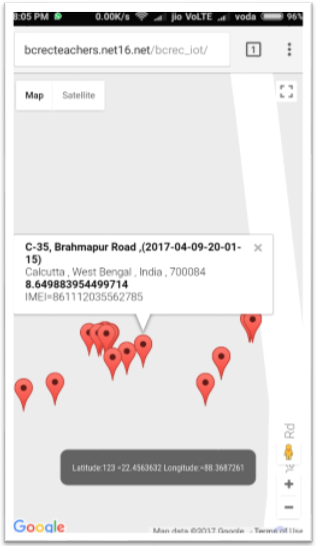
\includegraphics[width=5cm]{5.png}}
	\hfill
	\caption{User Interface}
\end{figure}

\section{Results}
The app is tested in Kolkata and Bardhaman region.


\begin{figure}[!htbp]
	\centering
	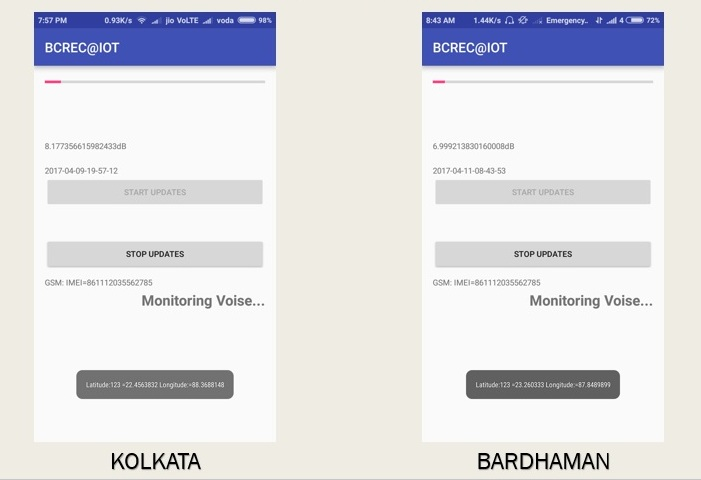
\includegraphics[width=0.9\textwidth]{6.jpg}
	\label{fig:Working of Android App}
	\caption{Working of Android App}
\end{figure}


\vspace{0.2in}
We have tested our application in Kolkata, Bardhaman and    Durgapur. In the figure, it displays the date-time, amplitude, latitude, longitude and IMEI no. of the android device.

\begin{figure}[!htbp]
	\centering
	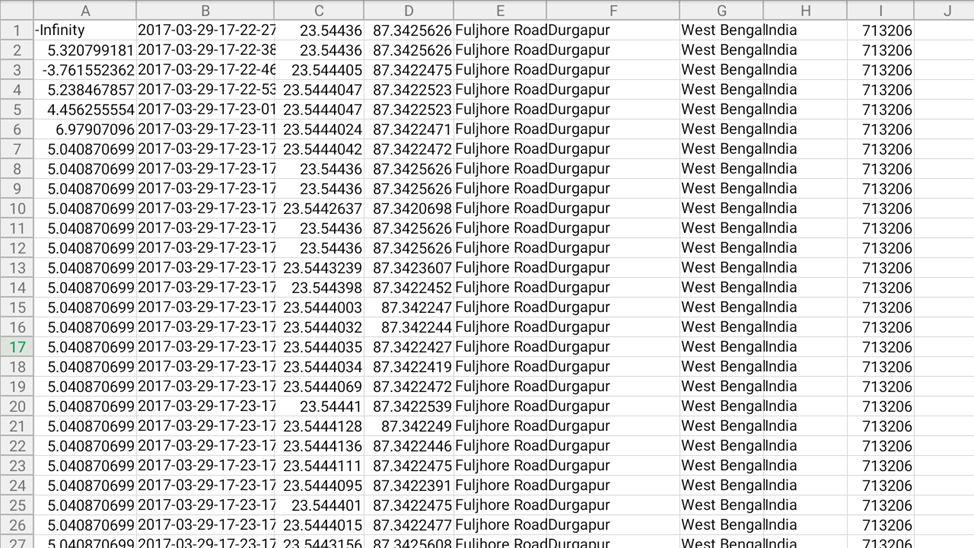
\includegraphics[width=0.9\textwidth]{7.png}
	\label{fig:Data Generated by the App}
	\caption{Data Generated by the App}
\end{figure}

The above figure 6.6 shows the log file which is stored in the SD card of the android device. All the data which will be displayed in the Google Map is written in rows and columns. Column A represents amplitude, B represents date-time, C and D represents latitude and longitude respectively, E represents IMEI number of the android device and F, G, H, I, J represents the address of the location. 

\begin{figure}[!htbp]
	\centering
	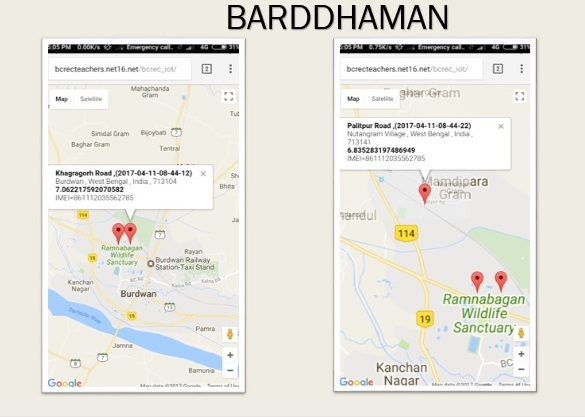
\includegraphics[width=0.6\textwidth]{8.jpg}
	\label{fig:Result Displayed to User}
	\caption{Result Displayed to User}
\end{figure}

In the figure 6.2, the marker is plotted on the Google Map at every given location (according to the values of their latitude And longitude). The corresponding date-time value, amplitude value, address of the location and IMEI of the Android device is also displayed on the Google Map.

\section{Future Scope}
\begin{itemize}
	\item \textbf{GPS Point}: We found the problem that multiple markers are pointing to particular point on the Google Map .So this problem needs to solve in future.
	\item \textbf{Mobile Sensor: }Every mobile sensor has its own specification and configuration. Data we are collecting is varying from device to device. We are getting the different data from different device for particular place. So this problem needs to resolve in future.
	
\end{itemize}
